% Options for packages loaded elsewhere
\PassOptionsToPackage{unicode}{hyperref}
\PassOptionsToPackage{hyphens}{url}
%
\documentclass[
]{article}
\usepackage{amsmath,amssymb}
\usepackage{iftex}
\ifPDFTeX
  \usepackage[T1]{fontenc}
  \usepackage[utf8]{inputenc}
  \usepackage{textcomp} % provide euro and other symbols
\else % if luatex or xetex
  \usepackage{unicode-math} % this also loads fontspec
  \defaultfontfeatures{Scale=MatchLowercase}
  \defaultfontfeatures[\rmfamily]{Ligatures=TeX,Scale=1}
\fi
\usepackage{lmodern}
\ifPDFTeX\else
  % xetex/luatex font selection
\fi
% Use upquote if available, for straight quotes in verbatim environments
\IfFileExists{upquote.sty}{\usepackage{upquote}}{}
\IfFileExists{microtype.sty}{% use microtype if available
  \usepackage[]{microtype}
  \UseMicrotypeSet[protrusion]{basicmath} % disable protrusion for tt fonts
}{}
\makeatletter
\@ifundefined{KOMAClassName}{% if non-KOMA class
  \IfFileExists{parskip.sty}{%
    \usepackage{parskip}
  }{% else
    \setlength{\parindent}{0pt}
    \setlength{\parskip}{6pt plus 2pt minus 1pt}}
}{% if KOMA class
  \KOMAoptions{parskip=half}}
\makeatother
\usepackage{xcolor}
\usepackage[margin=1in]{geometry}
\usepackage{color}
\usepackage{fancyvrb}
\newcommand{\VerbBar}{|}
\newcommand{\VERB}{\Verb[commandchars=\\\{\}]}
\DefineVerbatimEnvironment{Highlighting}{Verbatim}{commandchars=\\\{\}}
% Add ',fontsize=\small' for more characters per line
\usepackage{framed}
\definecolor{shadecolor}{RGB}{248,248,248}
\newenvironment{Shaded}{\begin{snugshade}}{\end{snugshade}}
\newcommand{\AlertTok}[1]{\textcolor[rgb]{0.94,0.16,0.16}{#1}}
\newcommand{\AnnotationTok}[1]{\textcolor[rgb]{0.56,0.35,0.01}{\textbf{\textit{#1}}}}
\newcommand{\AttributeTok}[1]{\textcolor[rgb]{0.13,0.29,0.53}{#1}}
\newcommand{\BaseNTok}[1]{\textcolor[rgb]{0.00,0.00,0.81}{#1}}
\newcommand{\BuiltInTok}[1]{#1}
\newcommand{\CharTok}[1]{\textcolor[rgb]{0.31,0.60,0.02}{#1}}
\newcommand{\CommentTok}[1]{\textcolor[rgb]{0.56,0.35,0.01}{\textit{#1}}}
\newcommand{\CommentVarTok}[1]{\textcolor[rgb]{0.56,0.35,0.01}{\textbf{\textit{#1}}}}
\newcommand{\ConstantTok}[1]{\textcolor[rgb]{0.56,0.35,0.01}{#1}}
\newcommand{\ControlFlowTok}[1]{\textcolor[rgb]{0.13,0.29,0.53}{\textbf{#1}}}
\newcommand{\DataTypeTok}[1]{\textcolor[rgb]{0.13,0.29,0.53}{#1}}
\newcommand{\DecValTok}[1]{\textcolor[rgb]{0.00,0.00,0.81}{#1}}
\newcommand{\DocumentationTok}[1]{\textcolor[rgb]{0.56,0.35,0.01}{\textbf{\textit{#1}}}}
\newcommand{\ErrorTok}[1]{\textcolor[rgb]{0.64,0.00,0.00}{\textbf{#1}}}
\newcommand{\ExtensionTok}[1]{#1}
\newcommand{\FloatTok}[1]{\textcolor[rgb]{0.00,0.00,0.81}{#1}}
\newcommand{\FunctionTok}[1]{\textcolor[rgb]{0.13,0.29,0.53}{\textbf{#1}}}
\newcommand{\ImportTok}[1]{#1}
\newcommand{\InformationTok}[1]{\textcolor[rgb]{0.56,0.35,0.01}{\textbf{\textit{#1}}}}
\newcommand{\KeywordTok}[1]{\textcolor[rgb]{0.13,0.29,0.53}{\textbf{#1}}}
\newcommand{\NormalTok}[1]{#1}
\newcommand{\OperatorTok}[1]{\textcolor[rgb]{0.81,0.36,0.00}{\textbf{#1}}}
\newcommand{\OtherTok}[1]{\textcolor[rgb]{0.56,0.35,0.01}{#1}}
\newcommand{\PreprocessorTok}[1]{\textcolor[rgb]{0.56,0.35,0.01}{\textit{#1}}}
\newcommand{\RegionMarkerTok}[1]{#1}
\newcommand{\SpecialCharTok}[1]{\textcolor[rgb]{0.81,0.36,0.00}{\textbf{#1}}}
\newcommand{\SpecialStringTok}[1]{\textcolor[rgb]{0.31,0.60,0.02}{#1}}
\newcommand{\StringTok}[1]{\textcolor[rgb]{0.31,0.60,0.02}{#1}}
\newcommand{\VariableTok}[1]{\textcolor[rgb]{0.00,0.00,0.00}{#1}}
\newcommand{\VerbatimStringTok}[1]{\textcolor[rgb]{0.31,0.60,0.02}{#1}}
\newcommand{\WarningTok}[1]{\textcolor[rgb]{0.56,0.35,0.01}{\textbf{\textit{#1}}}}
\usepackage{graphicx}
\makeatletter
\newsavebox\pandoc@box
\newcommand*\pandocbounded[1]{% scales image to fit in text height/width
  \sbox\pandoc@box{#1}%
  \Gscale@div\@tempa{\textheight}{\dimexpr\ht\pandoc@box+\dp\pandoc@box\relax}%
  \Gscale@div\@tempb{\linewidth}{\wd\pandoc@box}%
  \ifdim\@tempb\p@<\@tempa\p@\let\@tempa\@tempb\fi% select the smaller of both
  \ifdim\@tempa\p@<\p@\scalebox{\@tempa}{\usebox\pandoc@box}%
  \else\usebox{\pandoc@box}%
  \fi%
}
% Set default figure placement to htbp
\def\fps@figure{htbp}
\makeatother
\setlength{\emergencystretch}{3em} % prevent overfull lines
\providecommand{\tightlist}{%
  \setlength{\itemsep}{0pt}\setlength{\parskip}{0pt}}
\setcounter{secnumdepth}{-\maxdimen} % remove section numbering
\usepackage{bookmark}
\IfFileExists{xurl.sty}{\usepackage{xurl}}{} % add URL line breaks if available
\urlstyle{same}
\hypersetup{
  pdftitle={Final project analysis},
  pdfauthor={Wen Du},
  hidelinks,
  pdfcreator={LaTeX via pandoc}}

\title{Final project analysis}
\author{Wen Du}
\date{2026-04-27}

\begin{document}
\maketitle

\begin{Shaded}
\begin{Highlighting}[]
\FunctionTok{library}\NormalTok{(tidyverse)}
\FunctionTok{library}\NormalTok{(broom)}
\end{Highlighting}
\end{Shaded}

\begin{enumerate}
\def\labelenumi{\arabic{enumi}.}
\tightlist
\item
  Load Data
\end{enumerate}

\begin{Shaded}
\begin{Highlighting}[]
\NormalTok{df }\OtherTok{\textless{}{-}} \FunctionTok{read\_csv}\NormalTok{(}\StringTok{"../data/data\_final\_project.csv"}\NormalTok{)}
\end{Highlighting}
\end{Shaded}

\begin{verbatim}
## Rows: 6868 Columns: 26
## -- Column specification --------------------------------------------------------
## Delimiter: ","
## chr  (6): source, pedon_id, order, latlon_q, horizon, horizon_type
## dbl (19): lat, lon, horizon_number, depth2, depth1, depth, bulk_density, bd_...
## lgl  (1): pedon_start
## 
## i Use `spec()` to retrieve the full column specification for this data.
## i Specify the column types or set `show_col_types = FALSE` to quiet this message.
\end{verbatim}

\begin{Shaded}
\begin{Highlighting}[]
\FunctionTok{glimpse}\NormalTok{(df)}
\end{Highlighting}
\end{Shaded}

\begin{verbatim}
## Rows: 6,868
## Columns: 26
## $ source         <chr> "SANBORN & MASSICOTTE 2010", "SANBORN & MASSICOTTE 2010~
## $ pedon_id       <chr> "BC09-04", "BC09-04", "BC09-04", "BC09-04", "BC09-04", ~
## $ order          <chr> "Gleyed Dystric Brunisol", "Gleyed Dystric Brunisol", "~
## $ lat            <dbl> 54.07572, 54.07572, 54.07572, 54.07572, 54.07572, 54.07~
## $ lon            <dbl> -131.6861, -131.6861, -131.6861, -131.6861, -131.6861, ~
## $ latlon_q       <chr> "HIGH", "HIGH", "HIGH", "HIGH", "HIGH", "HIGH", "HIGH",~
## $ horizon_number <dbl> 1, 2, 3, 4, 5, 6, 7, 1, 2, 3, 4, 5, 6, 7, 8, 1, 2, 3, 4~
## $ horizon        <chr> "Lv/S", "Fm", "Hh", "Aeg", "Bmg", "BC", "Cg", "Lv", "Fm~
## $ horizon_type   <chr> NA, NA, NA, NA, NA, NA, NA, NA, NA, NA, NA, NA, NA, NA,~
## $ depth2         <dbl> 7, 6, 2, 0, -3, -35, -60, 13, 12, 11, 0, -7, -25, -55, ~
## $ depth1         <dbl> 6, 2, 0, -3, -35, -60, -110, 12, 11, 0, -7, -25, -55, -~
## $ depth          <dbl> 1, 4, 2, 3, 32, 25, 50, 1, 1, 11, 7, 18, 30, 30, 50, 1,~
## $ bulk_density   <dbl> 0.16, 0.16, 0.16, 1.48, 1.59, 1.59, 1.47, 0.16, 0.16, 0~
## $ bd_method      <dbl> 0, 0, 0, 0, 0, 0, 0, 0, 0, 0, 0, 0, 0, 0, 0, 0, 0, 0, 0~
## $ cf             <dbl> 0, 0, 0, 0, 0, 0, 0, 0, 0, 0, 0, 0, 0, 0, 0, 0, 0, 0, 0~
## $ cf_method      <dbl> 2, 2, 2, 2, 2, 2, 2, 2, 2, 2, 2, 2, 2, 2, 2, 2, 2, 2, 2~
## $ cconc          <dbl> 53.95, 21.77, 41.50, 0.47, 0.21, 0.16, 0.18, 53.33, 50.~
## $ cconc_method   <dbl> 0, 0, 0, 0, 0, 0, 0, 0, 0, 0, 0, 0, 0, 0, 0, 0, 0, 0, 0~
## $ mineral_d      <dbl> 100, NA, NA, NA, NA, NA, NA, 100, NA, NA, NA, NA, NA, N~
## $ ff_d           <dbl> 7, NA, NA, NA, NA, NA, NA, 13, NA, NA, NA, NA, NA, NA, ~
## $ total_d        <dbl> 107, NA, NA, NA, NA, NA, NA, 113, NA, NA, NA, NA, NA, N~
## $ ccontent       <dbl> 863, 1393, 1328, 209, 1068, 636, 1323, 853, 812, 8779, ~
## $ total_c        <dbl> 6820, NA, NA, NA, NA, NA, NA, 13978, NA, NA, NA, NA, NA~
## $ ccontent_1m    <dbl> 863, 1393, 1328, 209, 1068, 636, 1058, 853, 812, 8779, ~
## $ total_c_1m     <dbl> 65.55, NA, NA, NA, NA, NA, NA, 138.16, NA, NA, NA, NA, ~
## $ pedon_start    <lgl> TRUE, FALSE, FALSE, FALSE, FALSE, FALSE, FALSE, TRUE, F~
\end{verbatim}

\begin{enumerate}
\def\labelenumi{\arabic{enumi}.}
\setcounter{enumi}{1}
\tightlist
\item
  Create Pedon-level Dataset
\end{enumerate}

\begin{Shaded}
\begin{Highlighting}[]
\NormalTok{pedon\_df }\OtherTok{\textless{}{-}}\NormalTok{ df }\SpecialCharTok{\%\textgreater{}\%}
  \FunctionTok{filter}\NormalTok{(pedon\_start }\SpecialCharTok{==} \ConstantTok{TRUE}\NormalTok{) }\SpecialCharTok{\%\textgreater{}\%}
  \FunctionTok{mutate}\NormalTok{(}
    \AttributeTok{order\_group =} \FunctionTok{case\_when}\NormalTok{(}
      \FunctionTok{str\_detect}\NormalTok{(order, }\FunctionTok{regex}\NormalTok{(}\StringTok{"Histosol|Folisol|Mesisol|Humisol|Cryo"}\NormalTok{, }\AttributeTok{ignore\_case =} \ConstantTok{TRUE}\NormalTok{)) }\SpecialCharTok{\textasciitilde{}} \StringTok{"Organic soils"}\NormalTok{,}
      \FunctionTok{str\_detect}\NormalTok{(order, }\FunctionTok{regex}\NormalTok{(}\StringTok{"Podzol"}\NormalTok{, }\AttributeTok{ignore\_case =} \ConstantTok{TRUE}\NormalTok{)) }\SpecialCharTok{\textasciitilde{}} \StringTok{"Podzol"}\NormalTok{,}
      \FunctionTok{str\_detect}\NormalTok{(order, }\FunctionTok{regex}\NormalTok{(}\StringTok{"Brunisol|Brunisolic"}\NormalTok{, }\AttributeTok{ignore\_case =} \ConstantTok{TRUE}\NormalTok{)) }\SpecialCharTok{\textasciitilde{}} \StringTok{"Brunisol"}\NormalTok{,}
      \FunctionTok{str\_detect}\NormalTok{(order, }\FunctionTok{regex}\NormalTok{(}\StringTok{"Gleysol|Gleysolic"}\NormalTok{, }\AttributeTok{ignore\_case =} \ConstantTok{TRUE}\NormalTok{)) }\SpecialCharTok{\textasciitilde{}} \StringTok{"Gleysol"}\NormalTok{,}
      \FunctionTok{str\_detect}\NormalTok{(order, }\FunctionTok{regex}\NormalTok{(}\StringTok{"Regosol|Regosolic"}\NormalTok{, }\AttributeTok{ignore\_case =} \ConstantTok{TRUE}\NormalTok{)) }\SpecialCharTok{\textasciitilde{}} \StringTok{"Regosol"}\NormalTok{,}
      \ConstantTok{TRUE} \SpecialCharTok{\textasciitilde{}} \StringTok{"Other"}
\NormalTok{    )}
\NormalTok{  ) }\SpecialCharTok{\%\textgreater{}\%}
  \FunctionTok{select}\NormalTok{(pedon\_id, order, order\_group, total\_c\_1m, lat) }\SpecialCharTok{\%\textgreater{}\%}
  \FunctionTok{filter}\NormalTok{(}\SpecialCharTok{!}\FunctionTok{is.na}\NormalTok{(total\_c\_1m), }\SpecialCharTok{!}\FunctionTok{is.na}\NormalTok{(order\_group))}

\CommentTok{\# check structure}
\FunctionTok{glimpse}\NormalTok{(pedon\_df)}
\end{Highlighting}
\end{Shaded}

\begin{verbatim}
## Rows: 1,283
## Columns: 5
## $ pedon_id    <chr> "BC09-04", "BC09-01", "BC09-02", "BC09-03", "BC09-06", "BC~
## $ order       <chr> "Gleyed Dystric Brunisol", "Gleyed Dystric Brunisol", "Pla~
## $ order_group <chr> "Brunisol", "Brunisol", "Podzol", "Podzol", "Podzol", "Oth~
## $ total_c_1m  <dbl> 65.55, 138.16, 348.89, 336.43, 474.28, 0.00, 978.84, 869.9~
## $ lat         <dbl> 54.07572, 54.02631, 54.02253, 54.07275, 54.02200, 54.06908~
\end{verbatim}

\begin{Shaded}
\begin{Highlighting}[]
\CommentTok{\# check sample sizes}
\NormalTok{pedon\_df }\SpecialCharTok{\%\textgreater{}\%} \FunctionTok{count}\NormalTok{(order)}
\end{Highlighting}
\end{Shaded}

\begin{verbatim}
## # A tibble: 56 x 2
##    order                               n
##    <chr>                           <int>
##  1 Brunisolic                        317
##  2 Duric Dystric Brunisol              2
##  3 Duric Ferro-Humic Podzol            7
##  4 Duric Humo-Ferric Podzol            3
##  5 Dystric Brunisol                    4
##  6 Ferro-Humic Podzol                 60
##  7 Folisol                            10
##  8 Folisol (but horizons like pod)     1
##  9 Gleyed Brunisolic Gray Luvisol      1
## 10 Gleyed Dystric Brunisol             2
## # i 46 more rows
\end{verbatim}

\begin{enumerate}
\def\labelenumi{\arabic{enumi}.}
\setcounter{enumi}{2}
\tightlist
\item
  Exploratory Analysis
\end{enumerate}

Boxplot: Soil Carbon by Soil Order

\begin{Shaded}
\begin{Highlighting}[]
\FunctionTok{ggplot}\NormalTok{(pedon\_df, }\FunctionTok{aes}\NormalTok{(}\AttributeTok{x =}\NormalTok{ order\_group, }\AttributeTok{y =}\NormalTok{ total\_c\_1m, }\AttributeTok{fill =}\NormalTok{ order\_group)) }\SpecialCharTok{+}
  \FunctionTok{geom\_boxplot}\NormalTok{(}\AttributeTok{outlier.shape =} \ConstantTok{NA}\NormalTok{) }\SpecialCharTok{+}
  \FunctionTok{geom\_jitter}\NormalTok{(}\AttributeTok{width =} \FloatTok{0.15}\NormalTok{, }\AttributeTok{alpha =} \FloatTok{0.1}\NormalTok{) }\SpecialCharTok{+}
  \FunctionTok{theme\_classic}\NormalTok{() }\SpecialCharTok{+}
  \FunctionTok{labs}\NormalTok{(}
    \AttributeTok{title =} \StringTok{"Soil Carbon by Soil Group"}\NormalTok{,}
    \AttributeTok{x =} \StringTok{"Soil Group"}\NormalTok{,}
    \AttributeTok{y =} \StringTok{"Total Carbon (0{-}1 m)"}
\NormalTok{  )}
\end{Highlighting}
\end{Shaded}

\pandocbounded{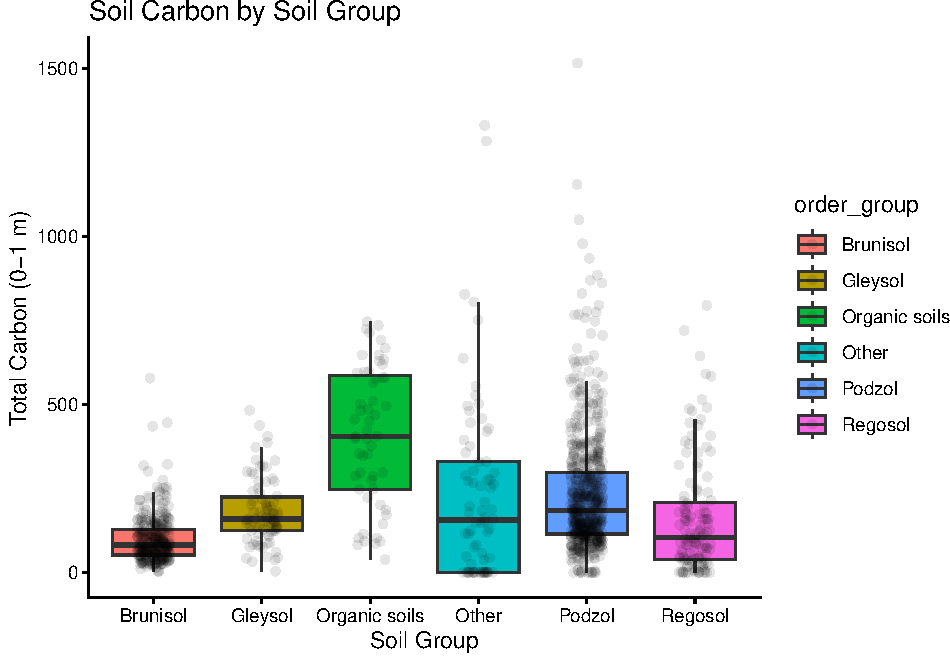
\includegraphics[keepaspectratio]{Final-project-analysis_files/Final-project-analysis_files/figure-latex/unnamed-chunk-3-1.pdf}}

\begin{enumerate}
\def\labelenumi{\arabic{enumi}.}
\setcounter{enumi}{3}
\tightlist
\item
  ANOVA: Does Carbon Differ Across Soil Orders?
\end{enumerate}

\begin{Shaded}
\begin{Highlighting}[]
\NormalTok{aov\_model }\OtherTok{\textless{}{-}} \FunctionTok{aov}\NormalTok{(total\_c\_1m }\SpecialCharTok{\textasciitilde{}}\NormalTok{ order\_group, }\AttributeTok{data =}\NormalTok{ pedon\_df)}
\FunctionTok{summary}\NormalTok{(aov\_model)}
\end{Highlighting}
\end{Shaded}

\begin{verbatim}
##               Df   Sum Sq Mean Sq F value Pr(>F)    
## order_group    5  6876360 1375272   52.64 <2e-16 ***
## Residuals   1277 33363385   26126                   
## ---
## Signif. codes:  0 '***' 0.001 '**' 0.01 '*' 0.05 '.' 0.1 ' ' 1
\end{verbatim}

Group Means

\begin{Shaded}
\begin{Highlighting}[]
\NormalTok{pedon\_df }\SpecialCharTok{\%\textgreater{}\%}
  \FunctionTok{group\_by}\NormalTok{(order) }\SpecialCharTok{\%\textgreater{}\%}
  \FunctionTok{summarise}\NormalTok{(}
    \AttributeTok{mean\_carbon =} \FunctionTok{mean}\NormalTok{(total\_c\_1m, }\AttributeTok{na.rm =} \ConstantTok{TRUE}\NormalTok{),}
    \AttributeTok{sd\_carbon =} \FunctionTok{sd}\NormalTok{(total\_c\_1m, }\AttributeTok{na.rm =} \ConstantTok{TRUE}\NormalTok{),}
    \AttributeTok{n =} \FunctionTok{n}\NormalTok{(),}
    \AttributeTok{.groups =} \StringTok{"drop"}
\NormalTok{  )}
\end{Highlighting}
\end{Shaded}

\begin{verbatim}
## # A tibble: 56 x 4
##    order                           mean_carbon sd_carbon     n
##    <chr>                                 <dbl>     <dbl> <int>
##  1 Brunisolic                             93.2      62.0   317
##  2 Duric Dystric Brunisol                161.       77.0     2
##  3 Duric Ferro-Humic Podzol              409.      259.      7
##  4 Duric Humo-Ferric Podzol              159.       56.1     3
##  5 Dystric Brunisol                      333.      177.      4
##  6 Ferro-Humic Podzol                    415.      271.     60
##  7 Folisol                               260.      258.     10
##  8 Folisol (but horizons like pod)       404.       NA       1
##  9 Gleyed Brunisolic Gray Luvisol        157.       NA       1
## 10 Gleyed Dystric Brunisol               102.       51.3     2
## # i 46 more rows
\end{verbatim}

\begin{enumerate}
\def\labelenumi{\arabic{enumi}.}
\setcounter{enumi}{4}
\tightlist
\item
  Regression: Carbon vs Latitude
\end{enumerate}

\begin{Shaded}
\begin{Highlighting}[]
\NormalTok{pedon\_df\_lat }\OtherTok{\textless{}{-}}\NormalTok{ pedon\_df }\SpecialCharTok{\%\textgreater{}\%}
  \FunctionTok{filter}\NormalTok{(lat }\SpecialCharTok{\textgreater{}} \DecValTok{40}\NormalTok{, lat }\SpecialCharTok{\textless{}} \DecValTok{65}\NormalTok{)}

\NormalTok{lm\_model }\OtherTok{\textless{}{-}} \FunctionTok{lm}\NormalTok{(total\_c\_1m }\SpecialCharTok{\textasciitilde{}}\NormalTok{ lat, }\AttributeTok{data =}\NormalTok{ pedon\_df\_lat)}
\FunctionTok{summary}\NormalTok{(lm\_model)}
\end{Highlighting}
\end{Shaded}

\begin{verbatim}
## 
## Call:
## lm(formula = total_c_1m ~ lat, data = pedon_df_lat)
## 
## Residuals:
##     Min      1Q  Median      3Q     Max 
## -275.19 -111.63  -46.66   61.64 1354.13 
## 
## Coefficients:
##             Estimate Std. Error t value Pr(>|t|)    
## (Intercept) -373.436     94.480  -3.953 8.16e-05 ***
## lat           10.952      1.819   6.021 2.26e-09 ***
## ---
## Signif. codes:  0 '***' 0.001 '**' 0.01 '*' 0.05 '.' 0.1 ' ' 1
## 
## Residual standard error: 174.5 on 1278 degrees of freedom
## Multiple R-squared:  0.02759,    Adjusted R-squared:  0.02683 
## F-statistic: 36.26 on 1 and 1278 DF,  p-value: 2.258e-09
\end{verbatim}

Plot Regression

\begin{Shaded}
\begin{Highlighting}[]
\CommentTok{\# 5. Regression: Carbon vs Latitude + Soil Order (Improved Model)}

\CommentTok{\# 先清理数据（过滤异常纬度）}
\NormalTok{pedon\_df\_mod }\OtherTok{\textless{}{-}}\NormalTok{ pedon\_df }\SpecialCharTok{\%\textgreater{}\%}
  \FunctionTok{filter}\NormalTok{(lat }\SpecialCharTok{\textgreater{}} \DecValTok{40}\NormalTok{, lat }\SpecialCharTok{\textless{}} \DecValTok{65}\NormalTok{)}

\CommentTok{\# 建立多元回归模型（关键升级）}
\NormalTok{lm\_model2 }\OtherTok{\textless{}{-}} \FunctionTok{lm}\NormalTok{(total\_c\_1m }\SpecialCharTok{\textasciitilde{}}\NormalTok{ lat }\SpecialCharTok{+}\NormalTok{ order\_group, }\AttributeTok{data =}\NormalTok{ pedon\_df\_mod)}

\CommentTok{\# 查看结果}
\FunctionTok{summary}\NormalTok{(lm\_model2)}
\end{Highlighting}
\end{Shaded}

\begin{verbatim}
## 
## Call:
## lm(formula = total_c_1m ~ lat + order_group, data = pedon_df_mod)
## 
## Residuals:
##     Min      1Q  Median      3Q     Max 
## -365.52  -97.31  -26.90   50.07 1296.03 
## 
## Coefficients:
##                          Estimate Std. Error t value Pr(>|t|)    
## (Intercept)              -132.357     90.468  -1.463 0.143708    
## lat                         4.494      1.759   2.554 0.010755 *  
## order_groupGleysol         78.749     19.939   3.949 8.26e-05 ***
## order_groupOrganic soils  286.895     24.925  11.510  < 2e-16 ***
## order_groupOther          132.262     20.879   6.335 3.29e-10 ***
## order_groupPodzol         132.915     11.054  12.024  < 2e-16 ***
## order_groupRegosol         59.831     16.994   3.521 0.000446 ***
## ---
## Signif. codes:  0 '***' 0.001 '**' 0.01 '*' 0.05 '.' 0.1 ' ' 1
## 
## Residual standard error: 161.4 on 1273 degrees of freedom
## Multiple R-squared:  0.1713, Adjusted R-squared:  0.1673 
## F-statistic: 43.84 on 6 and 1273 DF,  p-value: < 2.2e-16
\end{verbatim}

\begin{Shaded}
\begin{Highlighting}[]
\CommentTok{\# 更清晰的系数表（可用于报告）}
\FunctionTok{tidy}\NormalTok{(lm\_model2)}
\end{Highlighting}
\end{Shaded}

\begin{verbatim}
## # A tibble: 7 x 5
##   term                     estimate std.error statistic  p.value
##   <chr>                       <dbl>     <dbl>     <dbl>    <dbl>
## 1 (Intercept)               -132.       90.5      -1.46 1.44e- 1
## 2 lat                          4.49      1.76      2.55 1.08e- 2
## 3 order_groupGleysol          78.7      19.9       3.95 8.26e- 5
## 4 order_groupOrganic soils   287.       24.9      11.5  3.10e-29
## 5 order_groupOther           132.       20.9       6.33 3.29e-10
## 6 order_groupPodzol          133.       11.1      12.0  1.28e-31
## 7 order_groupRegosol          59.8      17.0       3.52 4.46e- 4
\end{verbatim}

\begin{Shaded}
\begin{Highlighting}[]
\CommentTok{\# 按 soil group 分开看趋势（强烈推荐）}
\FunctionTok{ggplot}\NormalTok{(pedon\_df\_mod, }\FunctionTok{aes}\NormalTok{(}\AttributeTok{x =}\NormalTok{ lat, }\AttributeTok{y =}\NormalTok{ total\_c\_1m, }\AttributeTok{color =}\NormalTok{ order\_group)) }\SpecialCharTok{+}
  \FunctionTok{geom\_point}\NormalTok{(}\AttributeTok{alpha =} \FloatTok{0.2}\NormalTok{, }\AttributeTok{size =} \DecValTok{1}\NormalTok{) }\SpecialCharTok{+}
  \FunctionTok{geom\_smooth}\NormalTok{(}\AttributeTok{method =} \StringTok{"lm"}\NormalTok{, }\AttributeTok{se =} \ConstantTok{FALSE}\NormalTok{) }\SpecialCharTok{+}
  \FunctionTok{facet\_wrap}\NormalTok{(}\SpecialCharTok{\textasciitilde{}}\NormalTok{ order\_group) }\SpecialCharTok{+}
  \FunctionTok{theme\_classic}\NormalTok{() }\SpecialCharTok{+}
  \FunctionTok{theme}\NormalTok{(}\AttributeTok{legend.position =} \StringTok{"none"}\NormalTok{)}\SpecialCharTok{+}
  \FunctionTok{labs}\NormalTok{(}\AttributeTok{subtitle =} \StringTok{"Slopes vary across soil groups, indicating weak but heterogeneous relationships"}\NormalTok{)}
\end{Highlighting}
\end{Shaded}

\begin{verbatim}
## `geom_smooth()` using formula = 'y ~ x'
\end{verbatim}

\pandocbounded{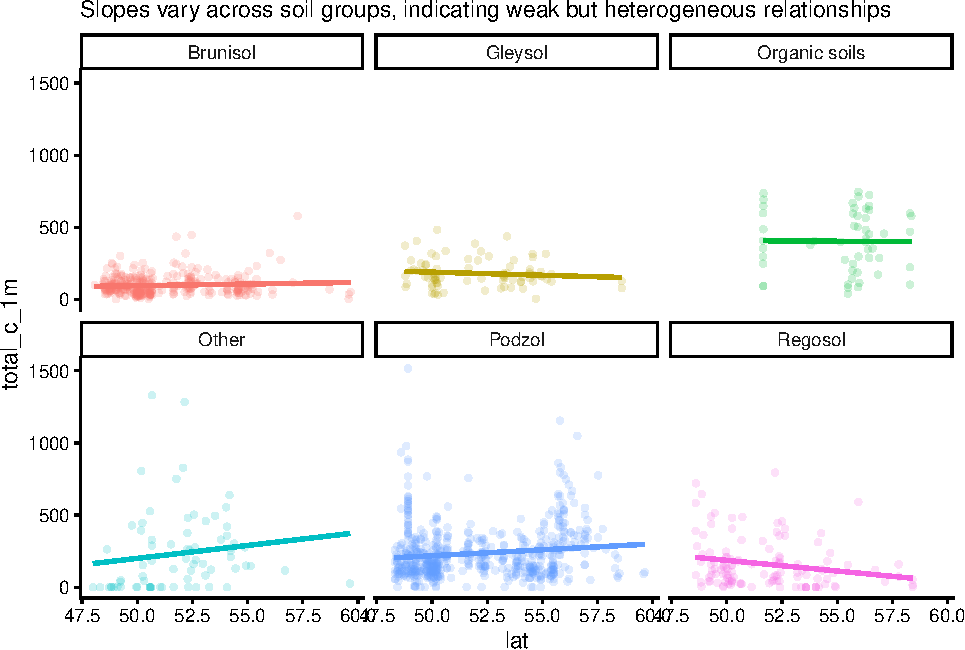
\includegraphics[keepaspectratio]{Final-project-analysis_files/Final-project-analysis_files/figure-latex/unnamed-chunk-7-1.pdf}}

\begin{Shaded}
\begin{Highlighting}[]
\NormalTok{lm\_model3 }\OtherTok{\textless{}{-}} \FunctionTok{lm}\NormalTok{(total\_c\_1m }\SpecialCharTok{\textasciitilde{}}\NormalTok{ lat }\SpecialCharTok{*}\NormalTok{ order\_group, }\AttributeTok{data =}\NormalTok{ pedon\_df\_mod)}

\FunctionTok{summary}\NormalTok{(lm\_model3)}
\end{Highlighting}
\end{Shaded}

\begin{verbatim}
## 
## Call:
## lm(formula = total_c_1m ~ lat * order_group, data = pedon_df_mod)
## 
## Residuals:
##     Min      1Q  Median      3Q     Max 
## -364.39  -93.44  -28.28   49.75 1307.42 
## 
## Coefficients:
##                              Estimate Std. Error t value Pr(>|t|)  
## (Intercept)                   -17.961    196.005  -0.092   0.9270  
## lat                             2.259      3.826   0.590   0.5551  
## order_groupGleysol            421.780    441.413   0.956   0.3395  
## order_groupOrganic soils      473.669    625.839   0.757   0.4493  
## order_groupOther             -676.508    496.139  -1.364   0.1730  
## order_groupPodzol            -175.371    229.329  -0.765   0.4446  
## order_groupRegosol            942.224    367.650   2.563   0.0105 *
## lat:order_groupGleysol         -6.557      8.504  -0.771   0.4408  
## lat:order_groupOrganic soils   -3.213     11.405  -0.282   0.7782  
## lat:order_groupOther           15.626      9.580   1.631   0.1031  
## lat:order_groupPodzol           5.966      4.458   1.338   0.1810  
## lat:order_groupRegosol        -17.025      7.119  -2.391   0.0169 *
## ---
## Signif. codes:  0 '***' 0.001 '**' 0.01 '*' 0.05 '.' 0.1 ' ' 1
## 
## Residual standard error: 160.6 on 1268 degrees of freedom
## Multiple R-squared:  0.1824, Adjusted R-squared:  0.1753 
## F-statistic: 25.71 on 11 and 1268 DF,  p-value: < 2.2e-16
\end{verbatim}

Horizon Contribution in Mineral Soils

\begin{Shaded}
\begin{Highlighting}[]
\NormalTok{mineral\_horizon\_summary }\OtherTok{\textless{}{-}}\NormalTok{ df }\SpecialCharTok{\%\textgreater{}\%}
  \FunctionTok{mutate}\NormalTok{(}
    \AttributeTok{order\_group =} \FunctionTok{case\_when}\NormalTok{(}
      \FunctionTok{str\_detect}\NormalTok{(order, }\FunctionTok{regex}\NormalTok{(}\StringTok{"Histosol|Folisol|Mesisol|Humisol|Cryo"}\NormalTok{, }\AttributeTok{ignore\_case =} \ConstantTok{TRUE}\NormalTok{)) }\SpecialCharTok{\textasciitilde{}} \StringTok{"Organic soils"}\NormalTok{,}
      \FunctionTok{str\_detect}\NormalTok{(order, }\FunctionTok{regex}\NormalTok{(}\StringTok{"Podzol"}\NormalTok{, }\AttributeTok{ignore\_case =} \ConstantTok{TRUE}\NormalTok{)) }\SpecialCharTok{\textasciitilde{}} \StringTok{"Podzol"}\NormalTok{,}
      \FunctionTok{str\_detect}\NormalTok{(order, }\FunctionTok{regex}\NormalTok{(}\StringTok{"Brunisol|Brunisolic"}\NormalTok{, }\AttributeTok{ignore\_case =} \ConstantTok{TRUE}\NormalTok{)) }\SpecialCharTok{\textasciitilde{}} \StringTok{"Brunisol"}\NormalTok{,}
      \FunctionTok{str\_detect}\NormalTok{(order, }\FunctionTok{regex}\NormalTok{(}\StringTok{"Gleysol|Gleysolic"}\NormalTok{, }\AttributeTok{ignore\_case =} \ConstantTok{TRUE}\NormalTok{)) }\SpecialCharTok{\textasciitilde{}} \StringTok{"Gleysol"}\NormalTok{,}
      \FunctionTok{str\_detect}\NormalTok{(order, }\FunctionTok{regex}\NormalTok{(}\StringTok{"Regosol|Regosolic"}\NormalTok{, }\AttributeTok{ignore\_case =} \ConstantTok{TRUE}\NormalTok{)) }\SpecialCharTok{\textasciitilde{}} \StringTok{"Regosol"}\NormalTok{,}
      \ConstantTok{TRUE} \SpecialCharTok{\textasciitilde{}} \StringTok{"Other"}
\NormalTok{    )}
\NormalTok{  ) }\SpecialCharTok{\%\textgreater{}\%}
  \FunctionTok{filter}\NormalTok{(order\_group }\SpecialCharTok{!=} \StringTok{"Organic soils"}\NormalTok{) }\SpecialCharTok{\%\textgreater{}\%}
  \FunctionTok{filter}\NormalTok{(}\SpecialCharTok{!}\FunctionTok{is.na}\NormalTok{(horizon\_type)) }\SpecialCharTok{\%\textgreater{}\%}
  \FunctionTok{group\_by}\NormalTok{(horizon\_type) }\SpecialCharTok{\%\textgreater{}\%}
  \FunctionTok{summarise}\NormalTok{(}
    \AttributeTok{total\_carbon =} \FunctionTok{sum}\NormalTok{(ccontent\_1m, }\AttributeTok{na.rm =} \ConstantTok{TRUE}\NormalTok{),}
    \AttributeTok{mean\_carbon =} \FunctionTok{mean}\NormalTok{(ccontent\_1m, }\AttributeTok{na.rm =} \ConstantTok{TRUE}\NormalTok{),}
    \AttributeTok{n =} \FunctionTok{n}\NormalTok{(),}
    \AttributeTok{.groups =} \StringTok{"drop"}
\NormalTok{  ) }\SpecialCharTok{\%\textgreater{}\%}
  \FunctionTok{mutate}\NormalTok{(}\AttributeTok{prop\_carbon =}\NormalTok{ total\_carbon }\SpecialCharTok{/} \FunctionTok{sum}\NormalTok{(total\_carbon))}

\NormalTok{mineral\_horizon\_summary}
\end{Highlighting}
\end{Shaded}

\begin{verbatim}
## # A tibble: 2 x 5
##   horizon_type total_carbon mean_carbon     n prop_carbon
##   <chr>               <dbl>       <dbl> <int>       <dbl>
## 1 Mineral          10678404       3620.  3169       0.632
## 2 Organic           6206694       2647.  2452       0.368
\end{verbatim}

\begin{enumerate}
\def\labelenumi{\arabic{enumi}.}
\setcounter{enumi}{6}
\tightlist
\item
  Notes
\end{enumerate}

\begin{itemize}
\tightlist
\item
  Analysis is conducted at the pedon level (independent observations)
\item
  Soil order is used instead of horizon-based classification
\item
  ANOVA tests group differences
\item
  Regression explores geographic trends
\end{itemize}

\end{document}
